\section{Simulation}\label{apx:sim}

\begin{lstlisting}[language=]
Version 4
SHEET 1 880 680
WIRE 176 32 32 32
WIRE 176 48 176 32
WIRE 32 144 32 32
WIRE 176 160 176 128
WIRE 176 256 176 224
WIRE 32 336 32 224
WIRE 176 336 176 320
WIRE 176 336 32 336
WIRE 176 368 176 336
FLAG 176 368 0
SYMBOL res 160 32 R0
SYMATTR InstName R1
SYMATTR Value 100
SYMATTR SpiceLine tol=1 pwr=0.1
SYMBOL cap 160 256 R0
SYMATTR InstName C1
SYMATTR Value 1µ
SYMATTR SpiceLine V=2.5 Irms=0 Rser=0 Lser=0
SYMBOL voltage 32 128 R0
WINDOW 3 -37 53 Right 2
WINDOW 123 0 0 Left 0
WINDOW 39 0 0 Left 0
SYMATTR InstName V1
SYMATTR Value 5
SYMBOL diode 160 160 R0
SYMATTR InstName D1
SYMATTR Value 1N4148
TEXT -66 366 Left 2 !.tran 1m startup
\end{lstlisting}

\section{\acrshort{pcb}}\label{apx:pcb}

\begin{figure}[H]
    \centering
    \begin{subfigure}{1.0\textwidth}
        \centering
        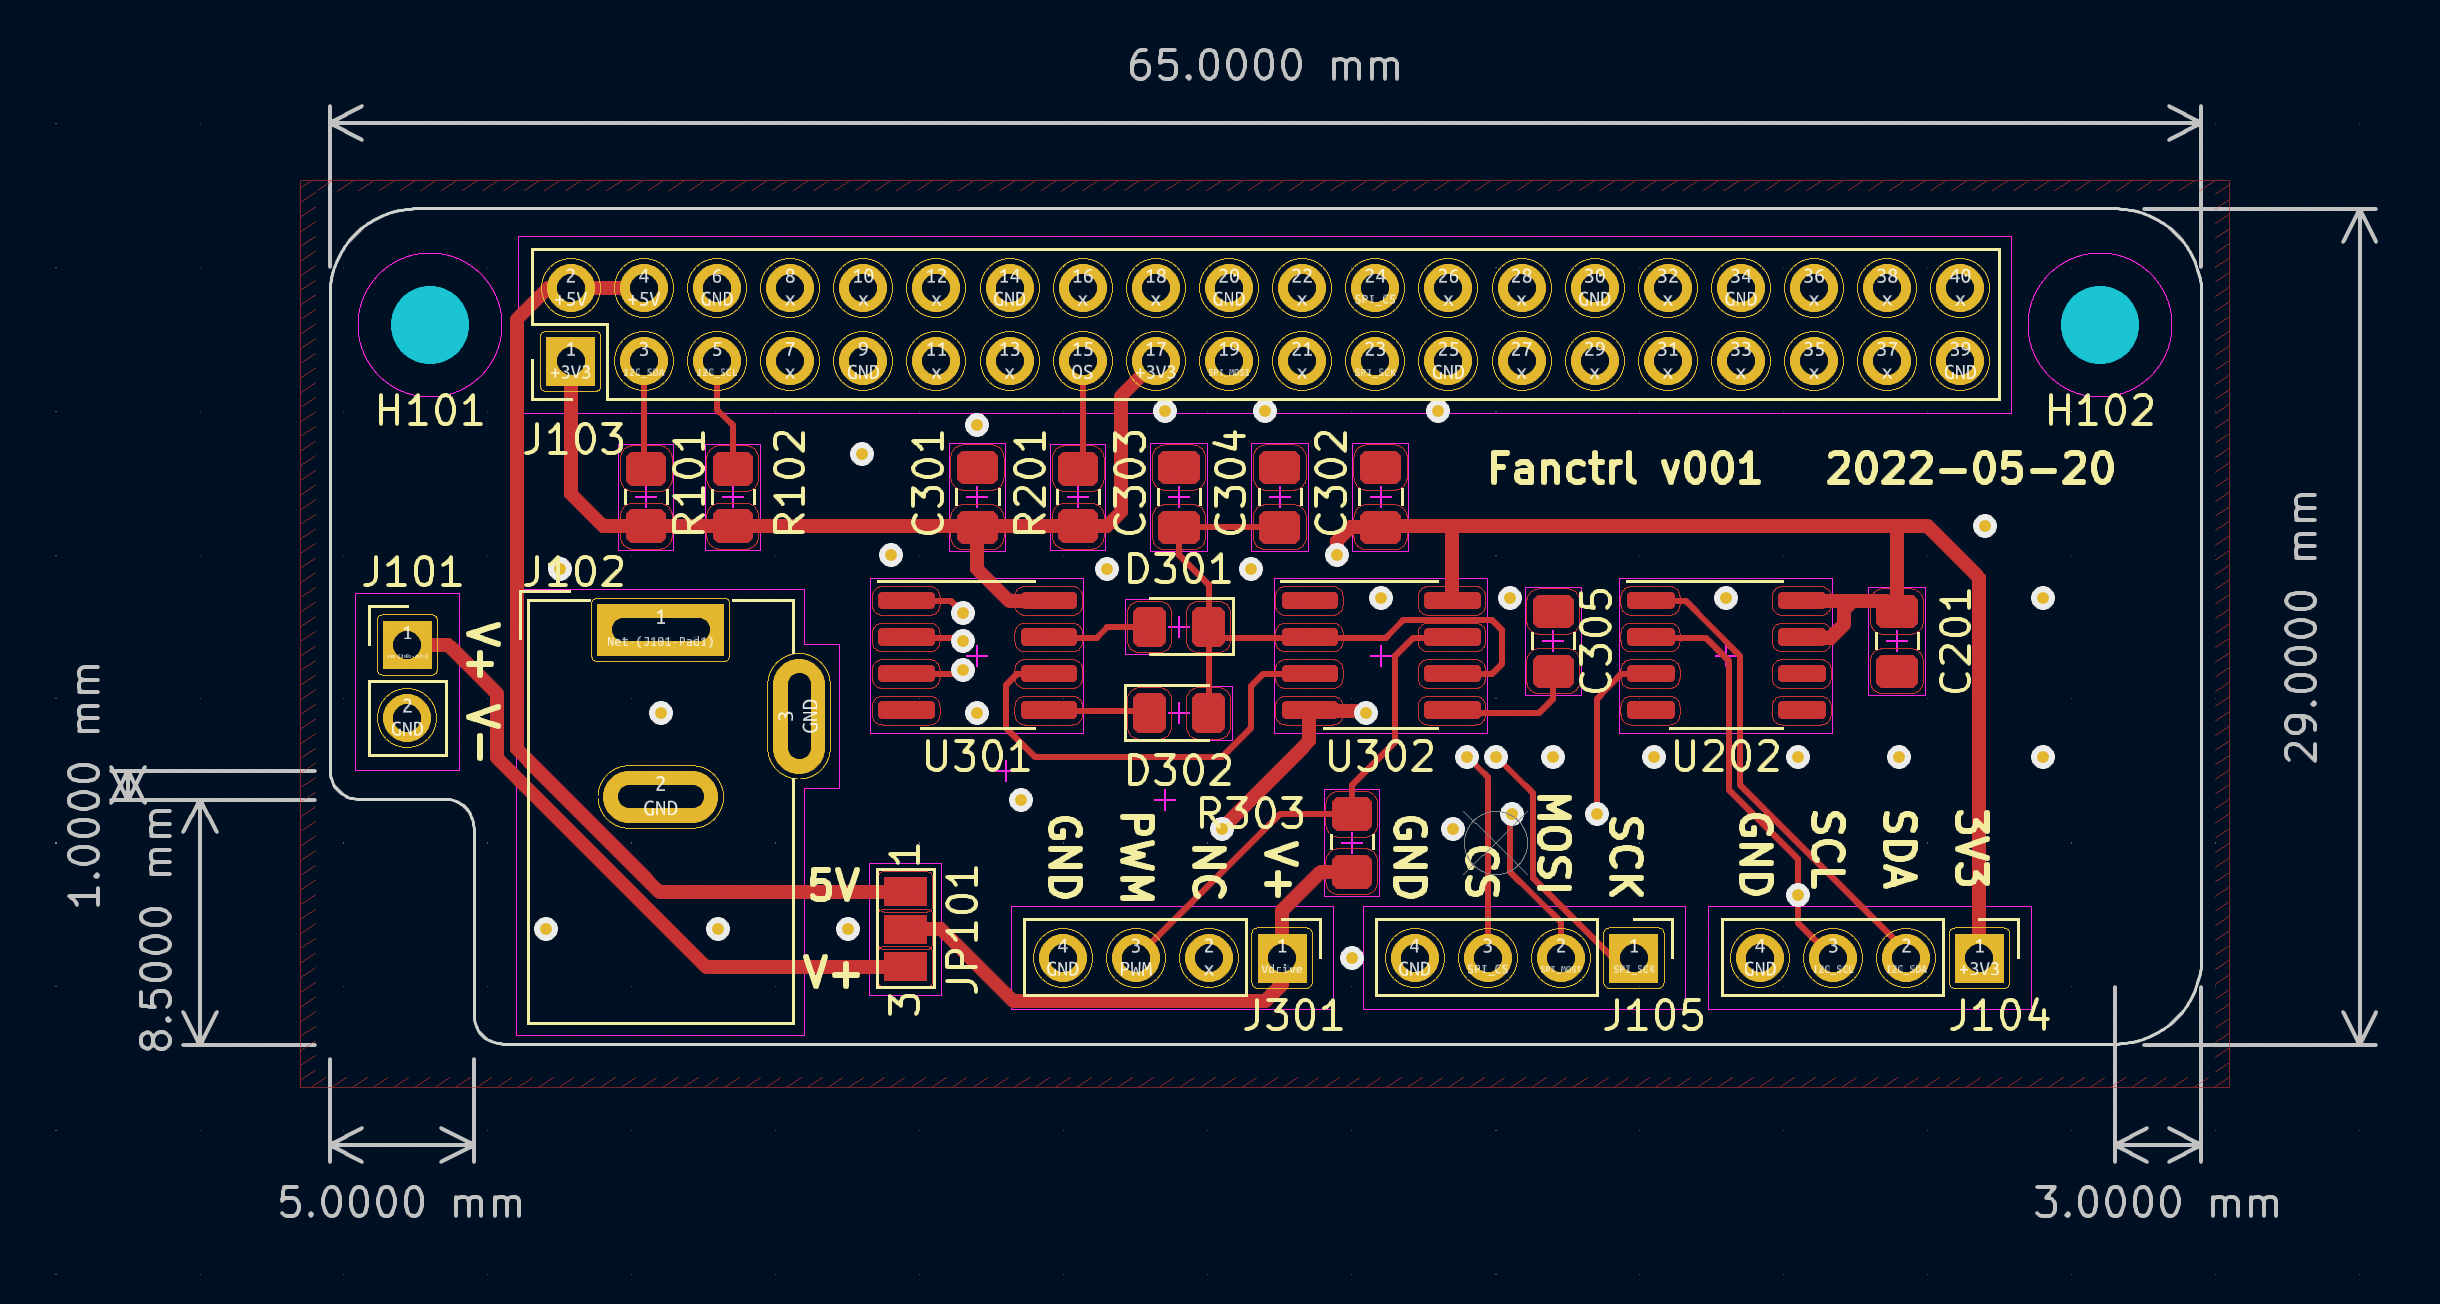
\includegraphics[width=15cm]{./pic/pcb-2d-top.png}
        \caption{TOP-Seite des \gls{pcb}}
    \end{subfigure}
    \begin{subfigure}{1.0\textwidth}
        \centering
        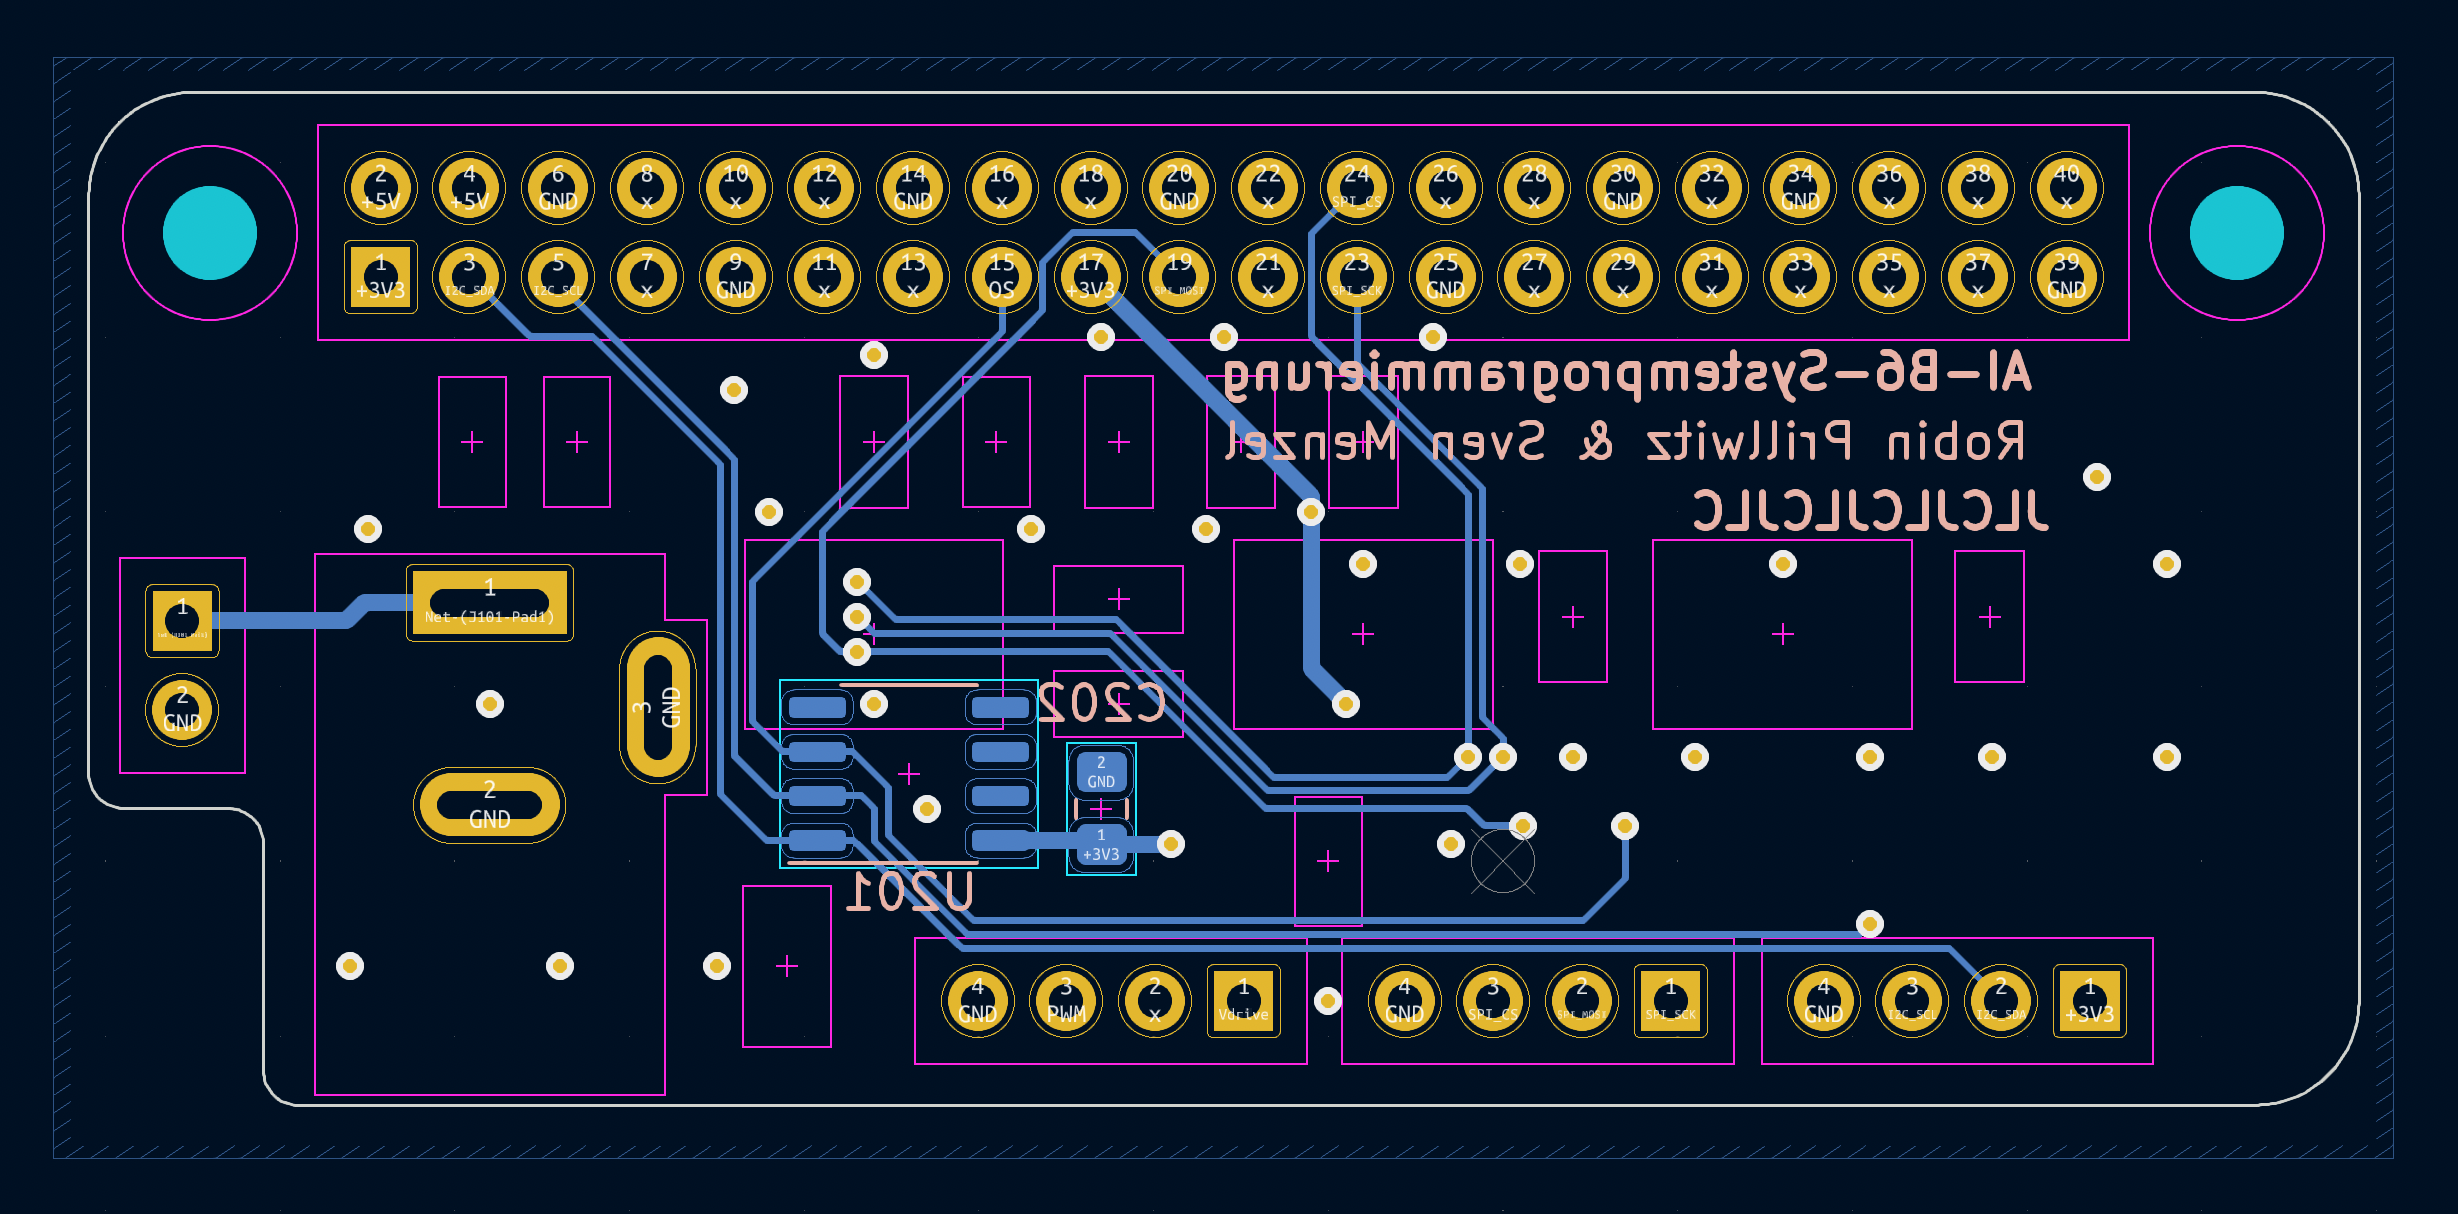
\includegraphics[width=15cm]{./pic/pcb-2d-bottom.png}
        \caption{BOTTOM-Seite des \gls{pcb}}
    \end{subfigure}
    \caption{2D Ansicht des \gls{pcb} aus \textit{KiCad}.}
    \label{fig:pcb-2d}
\end{figure}
\newpage

\begin{figure}[H]
    \centering
    \begin{subfigure}{1.0\textwidth}
        \centering
        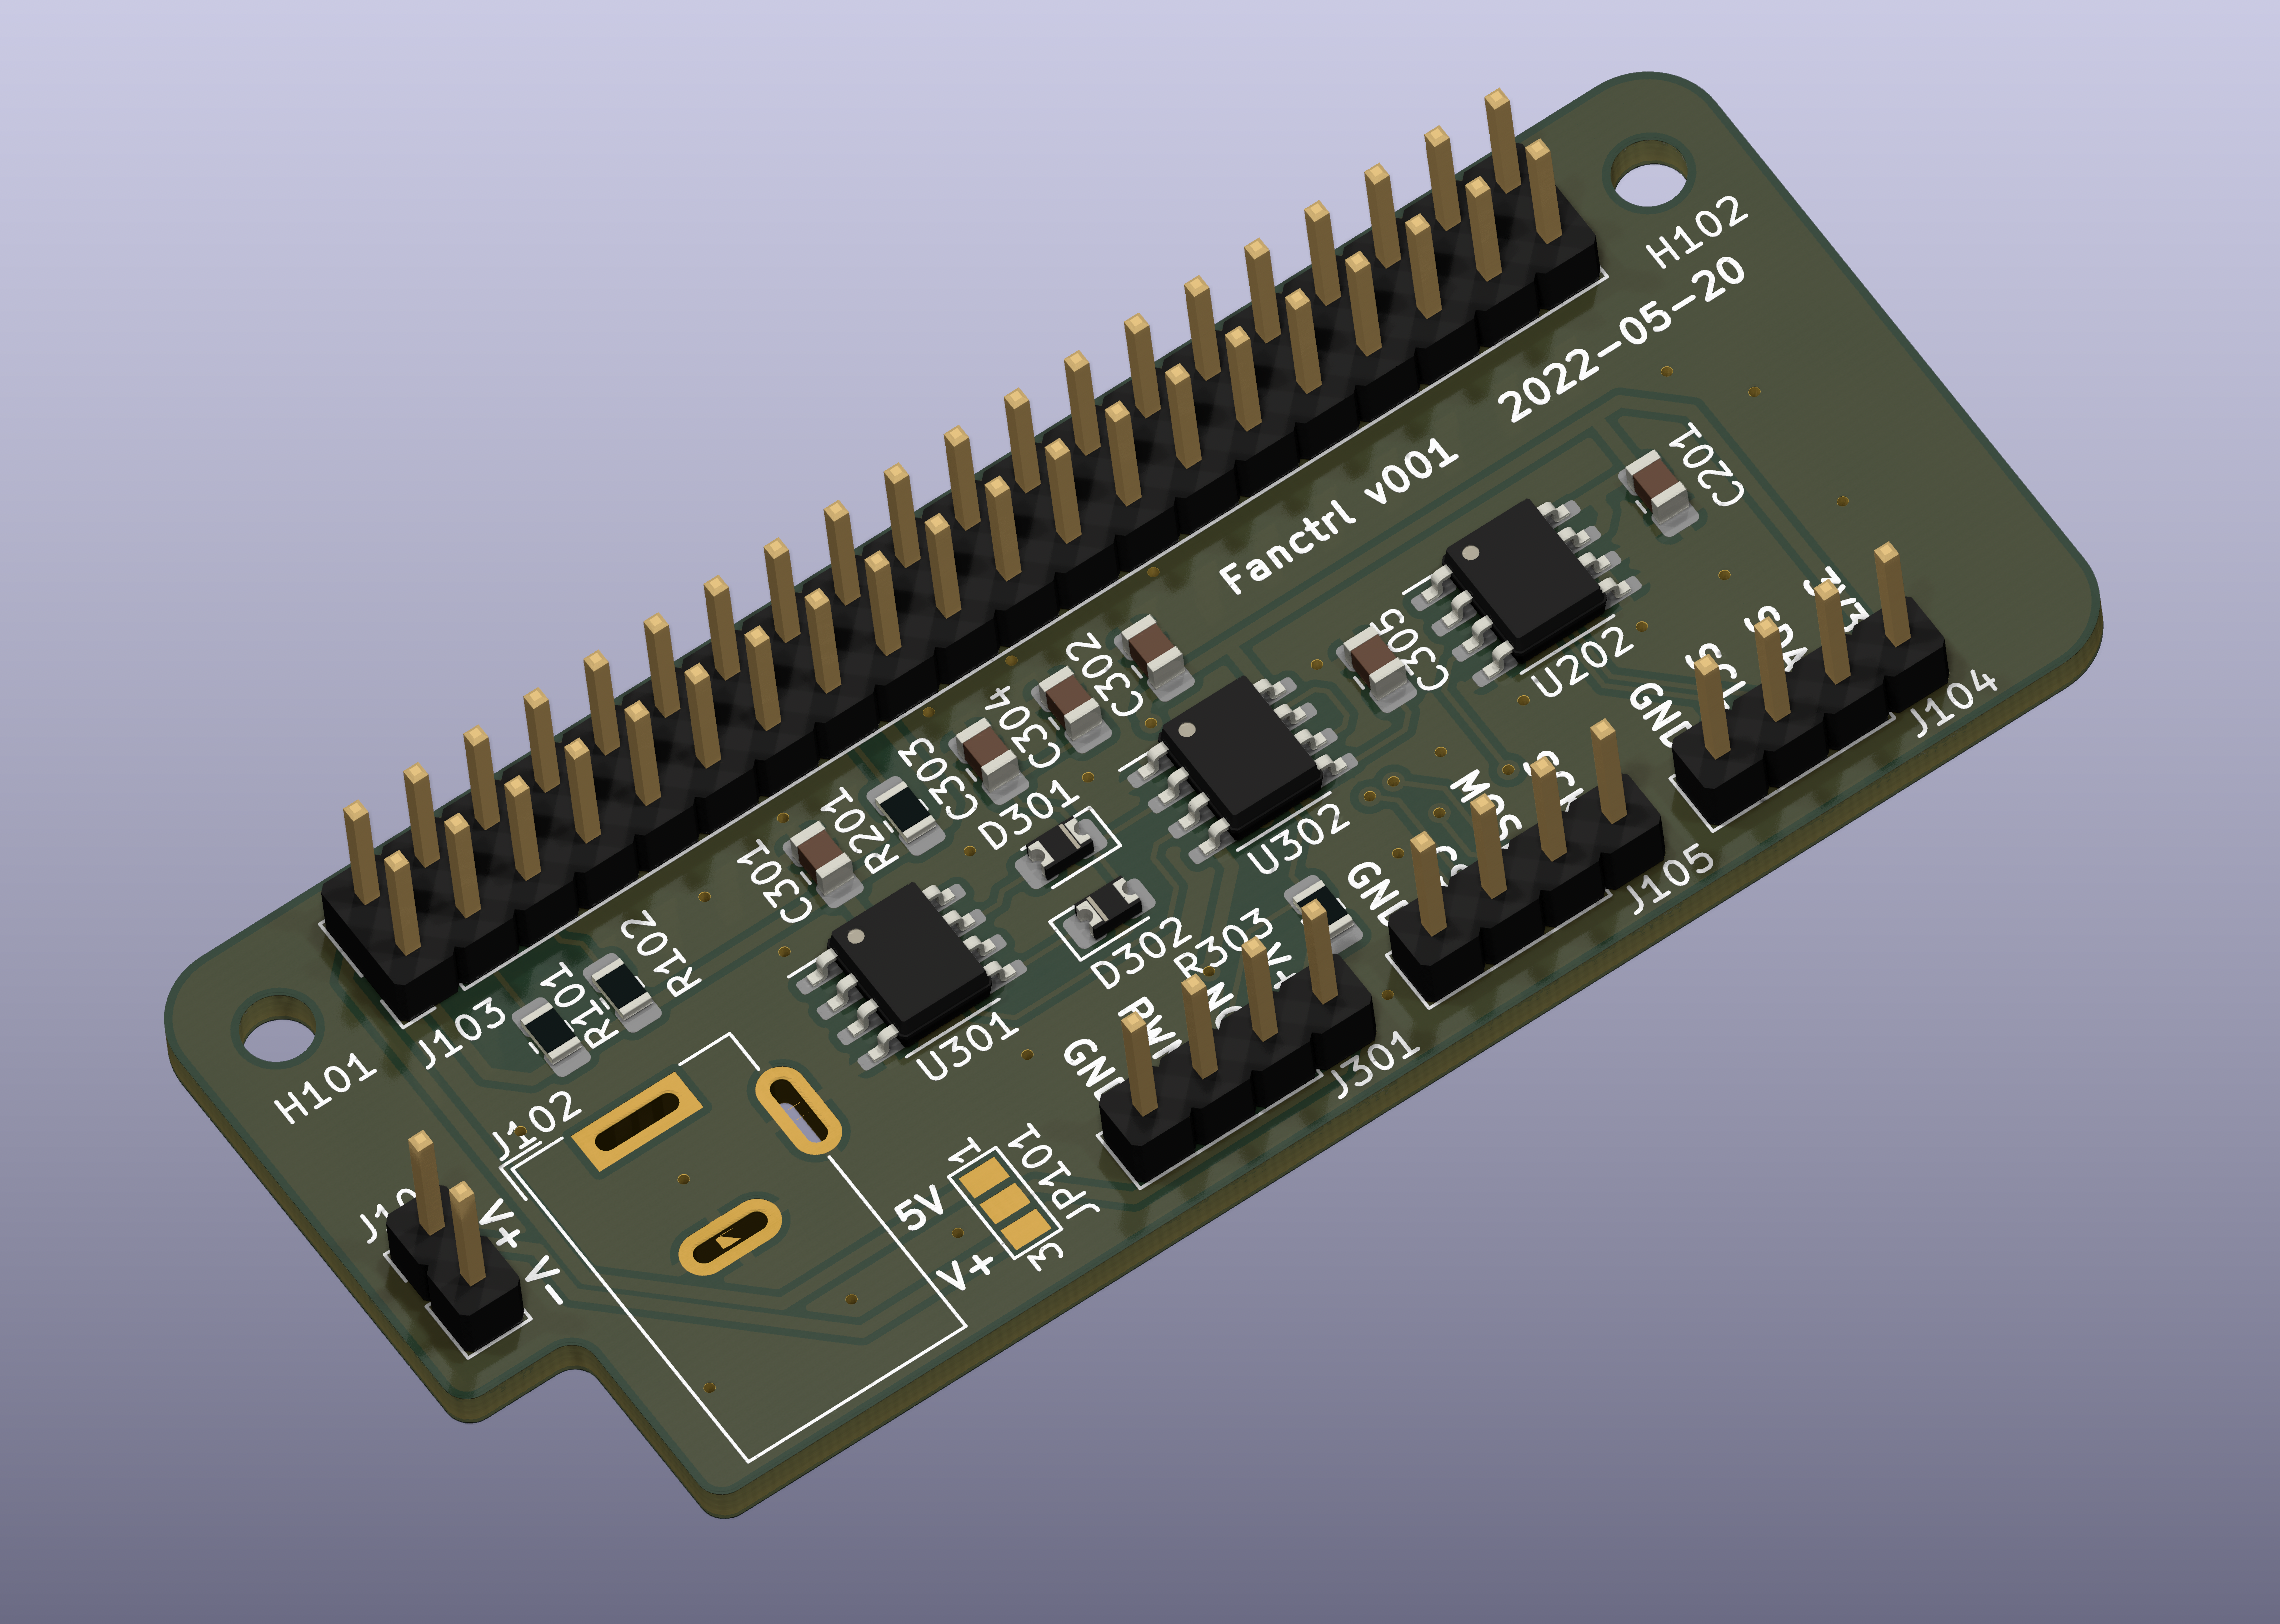
\includegraphics[width=15cm]{./pic/pcb-3d-top.png}
        \caption{TOP-Seite des \gls{pcb}}
    \end{subfigure}
    \begin{subfigure}{1.0\textwidth}
        \centering
        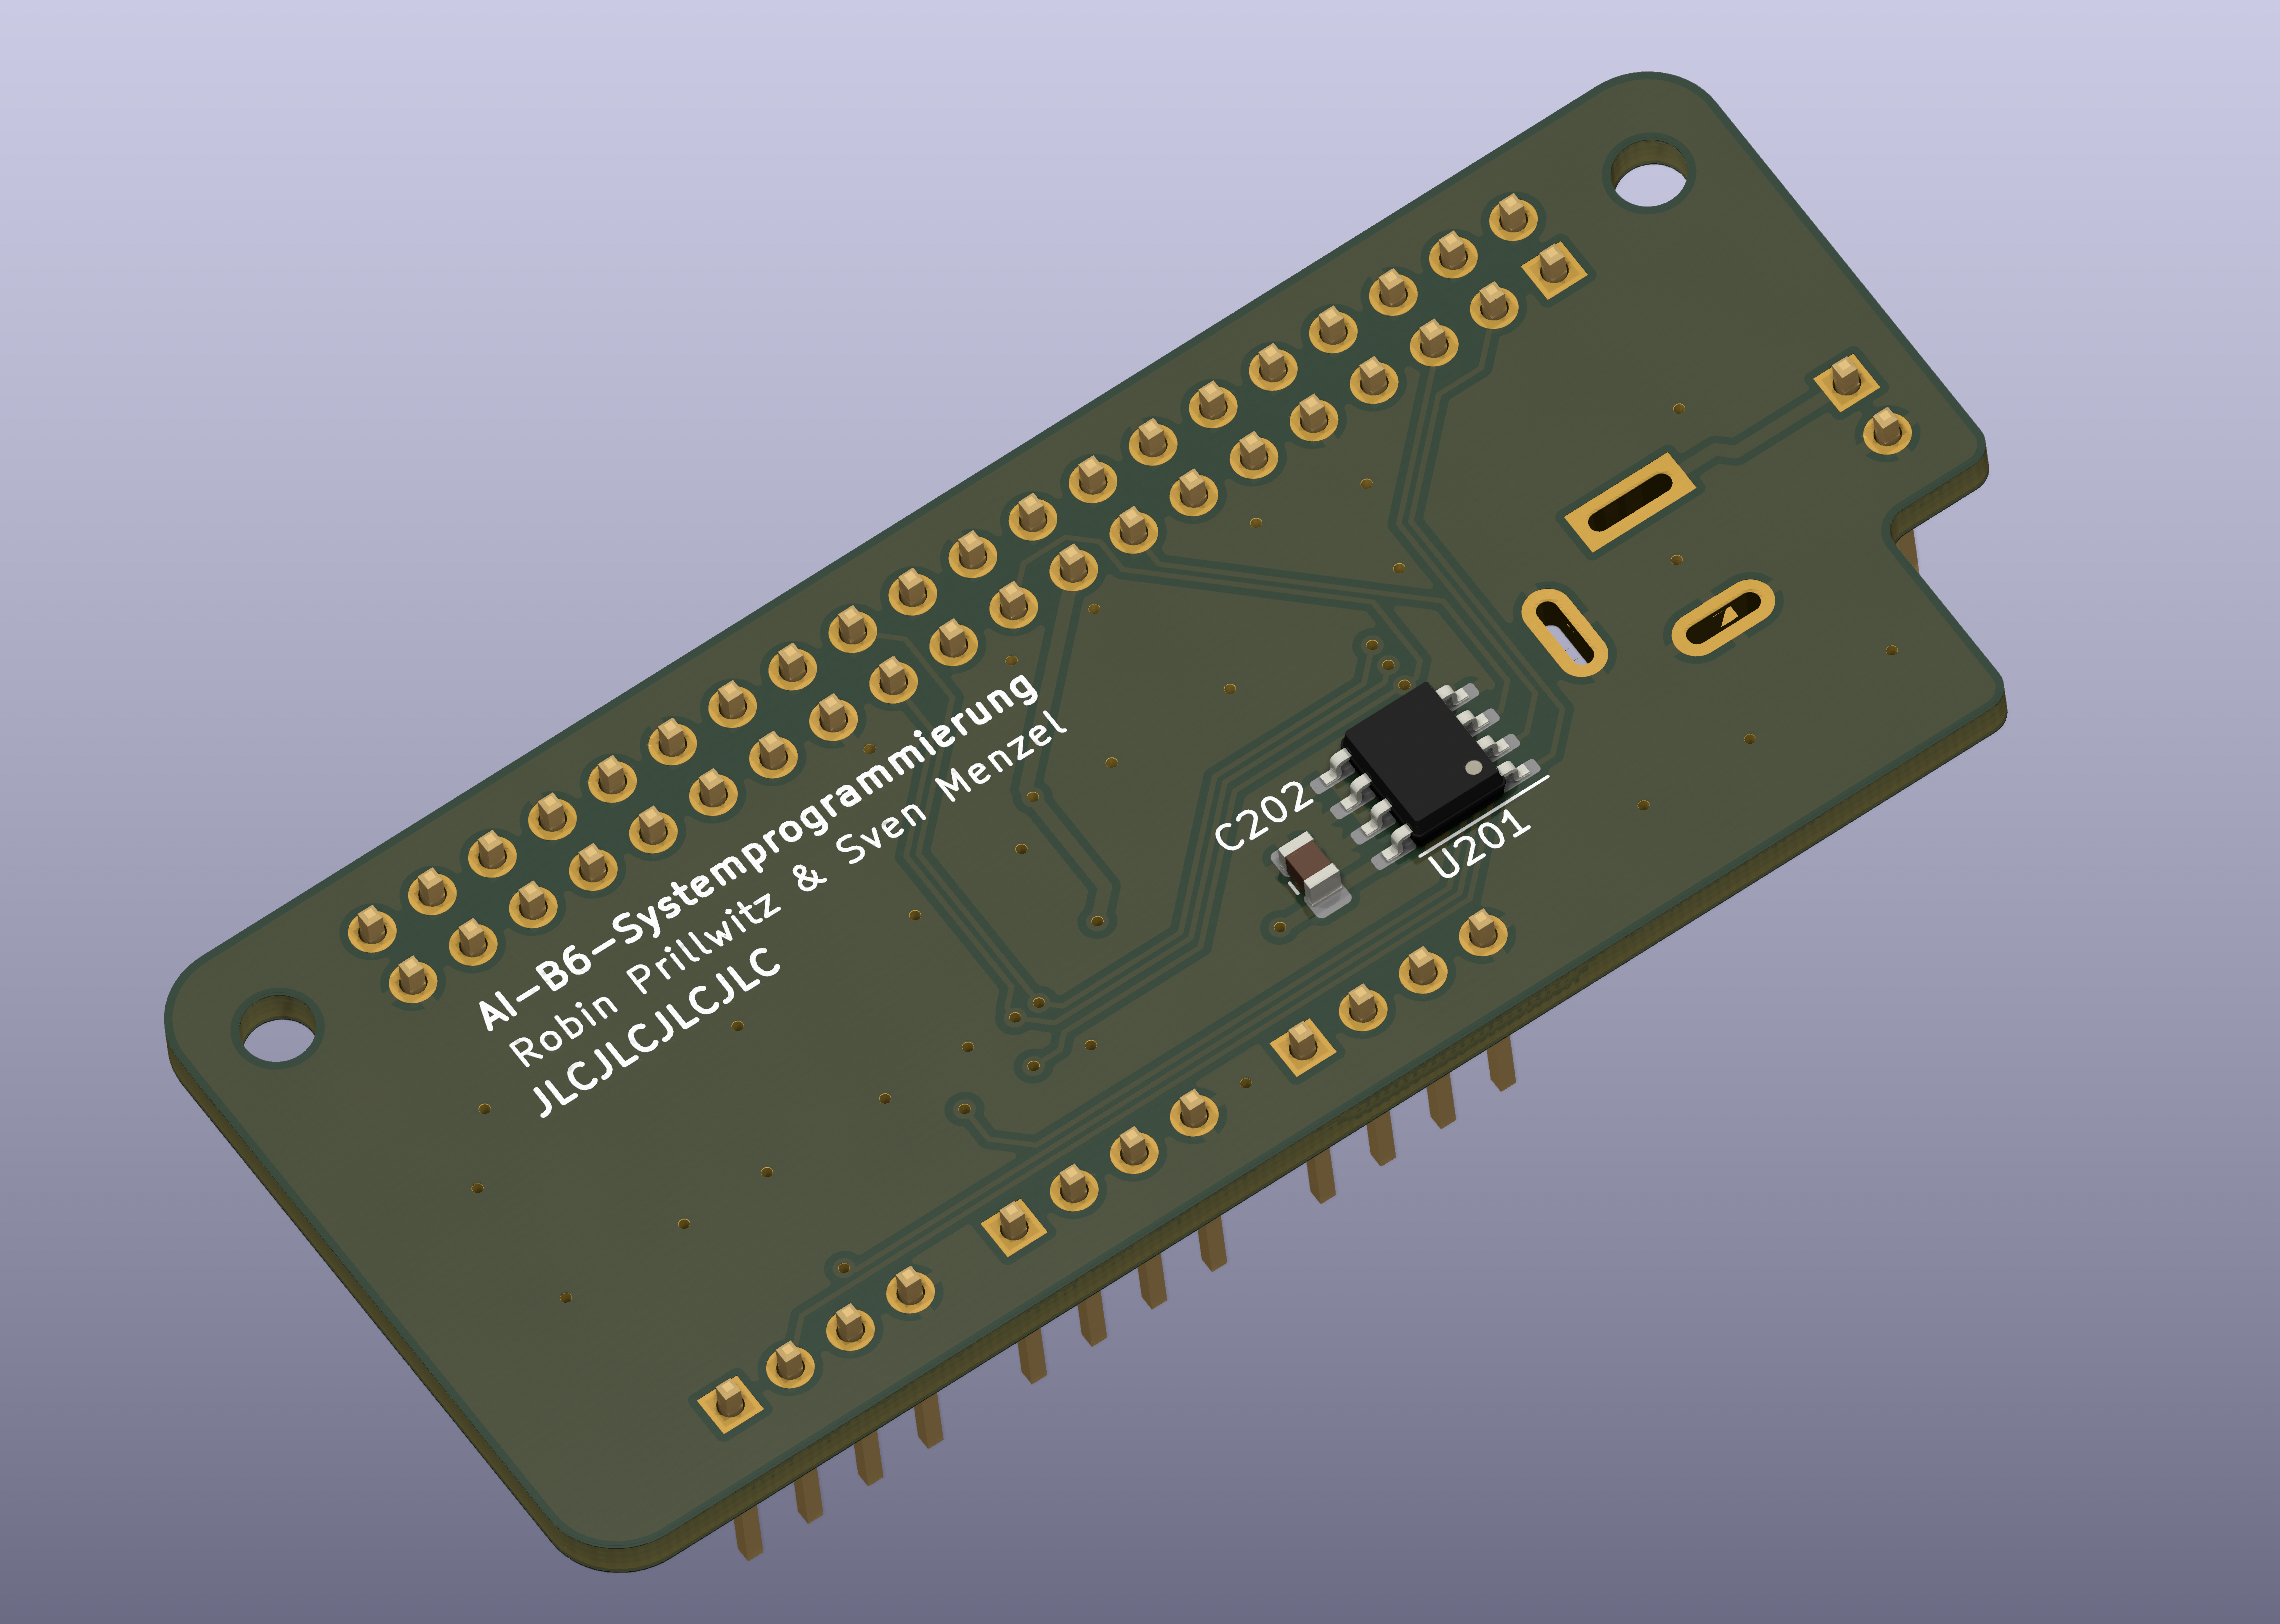
\includegraphics[width=15cm]{./pic/pcb-3d-bottom.png}
        \caption{BOTTOM-Seite des \gls{pcb}}
    \end{subfigure}
    \caption{3D Ansicht des \gls{pcb} aus \textit{KiCad}.}
    \label{fig:pcb-3d}
\end{figure}
\newpage

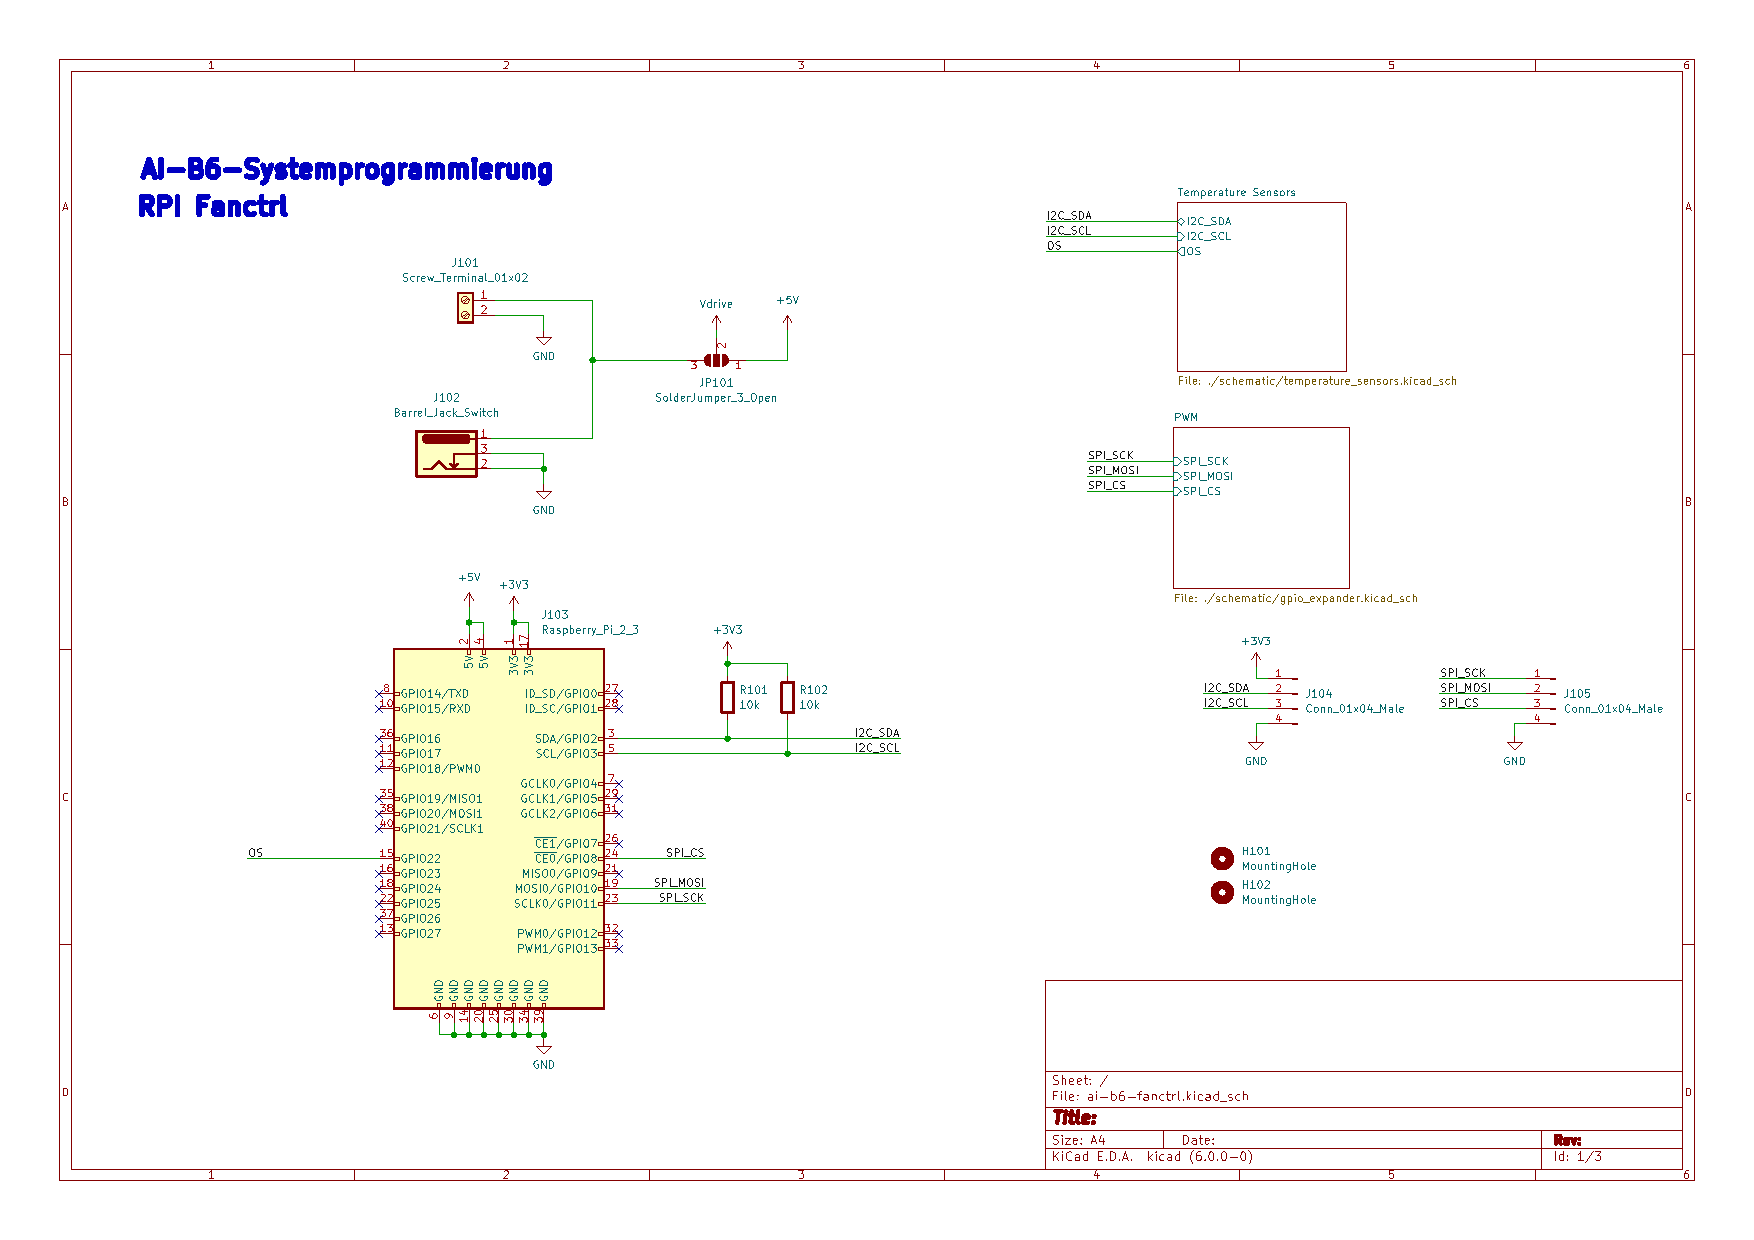
\includepdf[pages=-,scale=1.0,landscape=true,pagecommand={}]{./pic/ai-b6-fanctrl-schematic.pdf}
